\documentclass[12pt,letterpaper]{article}
\usepackage{graphicx,textcomp}
\usepackage{natbib}
\usepackage{setspace}
\usepackage{fullpage}
\usepackage{color}
\usepackage[reqno]{amsmath}
\usepackage{amsthm}
\usepackage{fancyvrb}
\usepackage{amssymb,enumerate}
\usepackage[all]{xy}
\usepackage{endnotes}
\usepackage{lscape}
\newtheorem{com}{Comment}
\usepackage{float}
\usepackage{hyperref}
\newtheorem{lem} {Lemma}
\newtheorem{prop}{Proposition}
\newtheorem{thm}{Theorem}
\newtheorem{defn}{Definition}
\newtheorem{cor}{Corollary}
\newtheorem{obs}{Observation}
\usepackage[compact]{titlesec}
\usepackage{dcolumn}
\usepackage{tikz}
\usetikzlibrary{arrows}
\usepackage{multirow}
\usepackage{xcolor}
\newcolumntype{.}{D{.}{.}{-1}}
\newcolumntype{d}[1]{D{.}{.}{#1}}
\definecolor{light-gray}{gray}{0.65}
\usepackage{url}
\usepackage{listings}
\usepackage{color}

\definecolor{codegreen}{rgb}{0,0.6,0}
\definecolor{codegray}{rgb}{0.5,0.5,0.5}
\definecolor{codepurple}{rgb}{0.58,0,0.82}
\definecolor{backcolour}{rgb}{0.95,0.95,0.92}

\lstdefinestyle{mystyle}{
	backgroundcolor=\color{backcolour},   
	commentstyle=\color{codegreen},
	keywordstyle=\color{magenta},
	numberstyle=\tiny\color{codegray},
	stringstyle=\color{codepurple},
	basicstyle=\footnotesize,
	breakatwhitespace=false,         
	breaklines=true,                 
	captionpos=b,                    
	keepspaces=true,                 
	numbers=left,                    
	numbersep=5pt,                  
	showspaces=false,                
	showstringspaces=false,
	showtabs=false,                  
	tabsize=2
}
\lstset{style=mystyle}
\newcommand{\Sref}[1]{Section~\ref{#1}}
\newtheorem{hyp}{Hypothesis}

\title{Problem Set 2}
\date{Due: October 14, 2024}
\author{Applied Stats/Quant Methods 1}

\begin{document}
	\maketitle
	\section*{Instructions}
\begin{itemize}
	\item Please show your work! You may lose points by simply writing in the answer. If the problem requires you to execute commands in \texttt{R}, please include the code you used to get your answers. Please also include the \texttt{.R} file that contains your code. If you are not sure if work needs to be shown for a particular problem, please ask.
	\item Your homework should be submitted electronically on GitHub.
	\item This problem set is due before 23:59 on Monday October 14, 2024. No late assignments will be accepted.

\end{itemize}

	
	\vspace{.5cm}
	\section*{Question 1: Political Science}
		\vspace{.25cm}
	The following table was created using the data from a study run in a major Latin American city.\footnote{Fried, Lagunes, and Venkataramani (2010). ``Corruption and Inequality at the Crossroad: A Multimethod Study of Bribery and Discrimination in Latin America. \textit{Latin American Research Review}. 45 (1): 76-97.} As part of the experimental treatment in the study, one employee of the research team was chosen to make illegal left turns across traffic to draw the attention of the police officers on shift. Two employee drivers were upper class, two were lower class drivers, and the identity of the driver was randomly assigned per encounter. The researchers were interested in whether officers were more or less likely to solicit a bribe from drivers depending on their class (officers use phrases like, ``We can solve this the easy way'' to draw a bribe). The table below shows the resulting data.

\newpage
\begin{table}[h!]
	\centering
	\begin{tabular}{l | c c c }
		& Not Stopped & Bribe requested & Stopped/given warning \\
		\\[-1.8ex] 
		\hline \\[-1.8ex]
		Upper class & 14 & 6 & 7 \\
		Lower class & 7 & 7 & 1 \\
		\hline
	\end{tabular}
\end{table}

\begin{enumerate}
	
	\item [(a)]
	Calculate the $\chi^2$ test statistic by hand/manually (even better if you can do "by hand" in \texttt{R}).\\
	
	The formula to find the $\chi^2$ test statistic is:
	(number of observances - number that is expected if the samples are fully independent )$^2$/number that is expected if the samples are fully independent
	
	To do so, I first need to calculate the number that is expected if the samples are fully independent ( f1e). In this context this is the amount of people (not) stopped or bribed in each class if the samples are fully independent, meaning if the class of the driver has no bearing on the behavior of the police.
	The formula for this number is:
	row total/grand total * column total
	
	Since there are going to be a lot of simple additions in my calculation of the $\chi^2$ test statistic I am going to try to make it less likely I forget part of an equation by already calculating the row/column/grand totals. 
	
	CODE FROM R!!
	
	Then I calculate f1e:
	
		CODE FROM R!!
		
	I get the following values: (ADD VALUES!!)
	Upper class - not stopped
	Upper class - bribe requested
	Upper class - stopped/given warning 
	Lower class - not stopped
	Lower class - bribe requested
	Lower class - stopped/given warning 
	
	With those number I can finally calculate my $\chi^2$ test statistic:
	CODE FROM R!!
	
	This mean that the $\chi^2$ test statistic equals 3.79. This number measures how much the observed data deviates from the expected data under the null hypothesis (which in this case is: the class of the driver does not affect how they are being treated by police, whether they were stopped or whether a bribe was requested). The chi-square test statistic quantifies the difference between observed data and what I would expect if the null hypothesis were true. The chi-square test statistic by itself shows the extent to which observed data deviates from what is expected under the null hypothesis, but it is not yet possible to fully interpret its meaning nor does it show if the result is statistically significant.
	
	\item [(b)]
	Now calculate the p-value from the test statistic you just created (in \texttt{R}).\footnote{Remember frequency should be $>$ 5 for all cells, but let's calculate the p-value here anyway.}  What do you conclude if $\alpha = 0.1$?\\
	
	I calculate the p-value using the pchisq() function in R. For this I need my saved chi-square value I calculated in (a), the degrees of freedom and I need to specify that I am interested in the upper tail (WHY?!) by clarifying lower.tail=FALSE. I can compute the degrees of freedom in the following way: (number of rows-1)*(number of columns-1). Seeing as we have two rows and three columns this results in (2-1)*(3-1)
	
	Function in R:
	CODE FROM R!!
	
	Since $\alpha = 0.1$?\\ and my alpha is larger than at 0.15, the effect is therefore not statistically significant , there is more evidence that like proposed in H0 the variables are independent.
	More formally: Based on the evidence provided by the p-value of the chi-square test statistic, we do not have sufficient evidence to reject our (implicit) null-hypothesis that officers are not more or less likely to solicit a bribe from drivers depending on their class. 
	Or, avoiding a double negative, we can say that we do not have sufficient evidence to accept our alternative hypothesis that officers are more or less likely to solicit a bribe from drivers depending on their class. There is no association between the class of the driver and whether or not an officer solicits a bribe (i.e., the variables are independent). 
	\newpage
	\item [(c)] Calculate the standardized residuals for each cell and put them in the table below.
	\vspace{1cm}
	
	the formula to calculate the standardized residuals, or more accurately the adjusted residuals (?) that we learned in class in the following:
	(fobserved-fexpected)/standard error (sqrt((1-row proportion)*(1- column proportion))
	meaning the observed value subtracted by the value one would expect under the null hypothesis divided by the square root of one minus the proportion of the total sample in a row multiplied by the proportion of the total sample in a column.
	
	First, to simplify matters for myself I calculate the row and column proportions.
	R CODE!!!
	
	Then I calculate the standardized residuals using the formula described above
	R CODE!!!
	
	\begin{table}[h]
		\centering
		\begin{tabular}{l | c c c }
			& Not Stopped & Bribe requested & Stopped/given warning \\
			\\[-1.8ex] 
			\hline \\[-1.8ex]
			Upper class  &0.3220306  & -1.641957 &1.523026  \\
			\\
			Lower class &-0.3220306  &1.641957   &-1.523026   \\
			
		\end{tabular}
	\end{table}
	
	
	\vspace{7cm}
	\item [(d)] How might the standardized residuals help you interpret the results?  
	
	The threshold under a 0.1: 
		NEW INTERPRETATION
		None of the standardized residuals exceed the threshold of ±1.645. meaning there are no statistically significant deviations in any of the cells. The observed and expected counts are generally close. This implied that class does not have a significant impact on whether officers solicit bribes or stop drivers.
	The residuals reinforce your earlier conclusion from the chi-square test: there's no strong evidence that the officers’ behavior (stopping or soliciting bribes) is influenced by the class of the drivers.
	
\end{enumerate}
\newpage

\section*{Question 2: Economics}
Chattopadhyay and Duflo were interested in whether women promote different policies than men.\footnote{Chattopadhyay and Duflo. (2004). ``Women as Policy Makers: Evidence from a Randomized Policy Experiment in India. \textit{Econometrica}. 72 (5), 1409-1443.} Answering this question with observational data is pretty difficult due to potential confounding problems (e.g. the districts that choose female politicians are likely to systematically differ in other aspects too). Hence, they exploit a randomized policy experiment in India, where since the mid-1990s, $\frac{1}{3}$ of village council heads have been randomly reserved for women. A subset of the data from West Bengal can be found at the following link: \url{https://raw.githubusercontent.com/kosukeimai/qss/master/PREDICTION/women.csv}\\

\noindent Each observation in the data set represents a village and there are two villages associated with one GP (i.e. a level of government is called "GP"). Figure~\ref{fig:women_desc} below shows the names and descriptions of the variables in the dataset. The authors hypothesize that female politicians are more likely to support policies female voters want. Researchers found that more women complain about the quality of drinking water than men. You need to estimate the effect of the reservation policy on the number of new or repaired drinking water facilities in the villages.
\vspace{.5cm}
\begin{figure}[h!]
	\caption{\footnotesize{Names and description of variables from Chattopadhyay and Duflo (2004).}}
	\vspace{.5cm}
	\centering
	\label{fig:women_desc}
	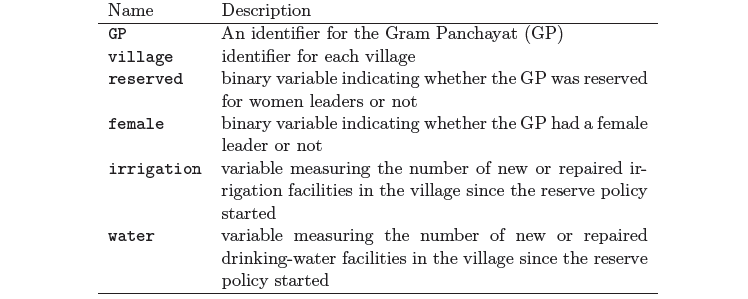
\includegraphics[width=1.1\textwidth]{women_desc.png}
\end{figure}		

\newpage
\begin{enumerate}
	\item [(a)] State a null and alternative (two-tailed) hypothesis. 
	
	\vspace{6cm}
	\item [(b)] Run a bivariate regression to test this hypothesis in \texttt{R} (include your code!).
	
	\vspace{6cm}
	\item [(c)] Interpret the coefficient estimate for reservation policy. 
\end{enumerate}

\end{document}
